\documentclass{article}
\usepackage{graphicx}
\usepackage{hyperref}
\usepackage{amsmath}
\usepackage{color}
\usepackage{cleveref}


\newcommand{\highlighttext}[1] {\textcolor{red}{#1}}


\title{Rebuttal: JMR-17-1184 (Research Paper), A Continuum of Optimal Tetrahelices between the Boerdijk-Coxeter Helix and a Planar-faced Tetrahelix}
\author{Robert L. Read \\
  Public Invention \\
    Email: \href{mailto:read.robert@gmail.com}{read.robert@gmail.com}   
	}

\date{\today}
% Hint: \title{what ever}, \author{who care} and \date{when ever} could stand 
% before or after the \begin{document} command 
% BUT the \maketitle command MUST come AFTER the \begin{document} command! 
\begin{document}

\maketitle

\section{Thanks}

The author wishes to thank the reviewers for their careful and attentive work, that has
significantly improved the paper. Each comment is responded
to below, on a point-by-point basis.

\section{Response to Reviewer \#1}

\subsection{Overview}

Slightly irregular edge lengths consisting the tetrahelix are introduced to develop one exact
revolution of the tetrahelix structure using the integer number of the tetrahedron in this paper.
Therefore, the efficient modeling of the tetrahelix using tetrahedral is proposed, and this research
can be applied to the robot or architecture field.

\subsection{Remarks}

In this paper, the optimality criterion is proposed to minimize the minimax which means the
difference between longest and shortest edge. For optimization, 7 conditions were considered.
However, these 7 conditions are just based on the author’s experience, but is not fully supported
by academic background such as kinematic measure to make any comparison between optimal
design and non-optimal design.

To parameterize the tetrahelix with respect to the rail angle, the relationship between one-hop edge,
two-hop edge, and rail edge is proposed.

The inradius of the tetrahelix was also calculated to consider the insertion of material inside the
tetrahelix.

The equitetrabeam is introduced as a special case that the rail angle is zero. It is proposed that
transformation from tetrahelix to equitetrabeam is possible by changing the minimax ratio about
16\%.

Overall, this paper is acceptable, but requires some revision. The following includes some comments.

\subsection{Modification}
\begin{itemize}
\item
The sentences of this paper need to be compact. Please read several times and then clean
the sentences.
``without loss of generality'' $\rightarrow$ ``generally''
\highlighttext{The term ``without loss of generality'' is being used specifically as mathematical jargon\cite{wiki:wolog} to represent an assumption allowed in a proof because of symmetry or an ability to make
  a choice that does not change the validity of the proof.
  However, because this was unclear to the reviewer, in order to clarify this, I have added the word ``assume'' to the first use of the phrase ``without loss of generality'' and the phrase ``By symmetry'' to the second use.
  }

\item
  The explanation for figure 8 can be erased by drawing the general case for figure 8.
  \highlighttext{Yes, you are correct, thank you, I have made the diagram (see \cref{fig:wobble}) more general and removed the
    disclaiming text.}
    \begin{figure}
     \centering
     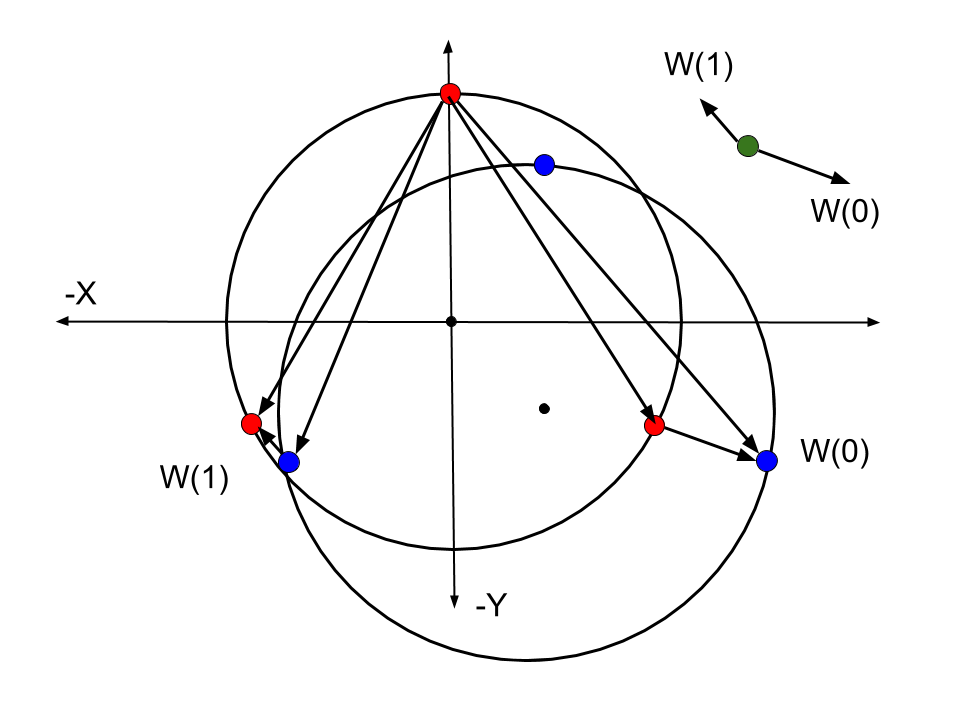
\includegraphics[width=0.45\textwidth]{figures/WobbleDiagram2.png}
     \caption{Wobble Vectors from Non-Coincident Axes}
  \label{fig:wobble}
\end{figure}
  \item
    Instead of sentence starting to ‘we……’ , the passive sentence is recommended.
    \highlighttext{
      I believe editorial opinion is somewhat divided\cite{firstperson} on the use of the word ``we'' when it is used to mean ``the author and the reader together'' as I have used it. Most editors do not prefer passive sentences in general.
      Nonetheless, in deference to the reviewer, I have searched the paper for each use of the word ``we'' and
      removed it in most, but not all cases.
      }
    \item 
 The following sentence is obscure. You'd better suggest a way to measure optimality using
 some kinematic indices :
\begin{quote}
 We have not yet proved that a two-class tetrahelix is optimal, but it suffices to show
that there exists such a better tetrahelix to show that different radii imply a suboptimal
tetrahelix.
\end{quote}

\highlighttext{
  The reviewer has generally noted that I may not have motivated my definition of ``optimality''
  strongly enough. To improve this, I have made some changes:
... displays a continuum of tetrahelices optimal \bf{
  in the sense of being
as regular as possible},
which is the main result of this
paper.
}

\highlighttext{
  Additionally, in the section on Optimal Tetrahelices, I have inserted the following sentence which helps to
  explain the definition of optimality:
  \bf{By maintaining all lengths as close to the same ``regular'' length as possible,
such as the mean length of the actuator,
one retains the greatest possible freedom of motion for the robot.}
  }

\highlighttext{This specific sentence has been clarified to show that ``not yet proved'' means
  ``not yet reached the proof in this paper of that fact that'' by changing the sentence to refer
  to the next theorem:
  \begin{quote}
  We have not yet {\em
proved theorem 3 which asserts} that a two-class tetrahelix is optimal, but it suffices to show that there
exists such a better tetrahelix to show that different radii imply a suboptimal
tetrahelix.
  \end{quote}
  I unfortunately am not sure how to relate this notion of optimality to kinematic indexes, but
  have attempted elsewhere to clarify why this definition of optimality is valuable for
  Tetrobot-style robots.
  }
\item 
 It is recommended to change:
 ``conincident'' $\rightarrow$ ``coincident''
 \highlighttext{Corrected--an embarrassing mistake in my spelling correction software.}
\item In page 3, after the eq. (4)
  In this formula, ``integral values of n'' $\rightarrow$ In this formula, ``integer values of n''
  \highlighttext{Corrected.}
  \item 
In eq. (23), need to be changed as

\begin{equation}
  \begin{split}
  \frac{\text{two-hop}(r)}{ \text{one-hop}(r)}  &=
  \frac{\sqrt{\frac{4}{9}  + r^2(g_{\rho}+ j_{\rho})}}
       {\sqrt{\frac{1}{9} +r^2(f_{\rho}+k_{\rho}) }} \text{.}
  \end{split}       
\end{equation}
$\rightarrow$ 
\begin{equation}
  \begin{split}
  \frac{\text{two-hop}(r)}{ \text{one-hop}(r)}  &=
  \frac{\sqrt{\frac{4}{9}  + r^2(g_{\rho}+ k_{\rho})}}
       {\sqrt{\frac{1}{9} +r^2(f_{\rho}+j_{\rho}) }} \text{.}
  \end{split}       
\end{equation}
\highlighttext{This has been corrected, thanks for the careful catch of an embarrassing mistake.}

\item 
- In page 8, the graph could not be observed through this following address,
https://github.com/PubInv/tetrahelix/blob/master/tetrahelix.nb . For user not using the
Mathematica, it is recommended to show the tendency of the graph of eq. (23) by setting
rail angle as 0, 15, and 30(deg).

\highlighttext{
  In order to make this clearer and avoid forcing the user to follow a link, I have included the graphic
  inline in the document with the following change to the relevant sentence:}

\begin{quote}

  By inspection of the graph of the derivative of this ratio rendered in \cref{fig:partialderivativediagram}
  observe that the partial derivative of this with respect to
radius $r$ is always negative, for any $\rho \leq \rho_{bc}$.

\begin{figure}
     \centering
     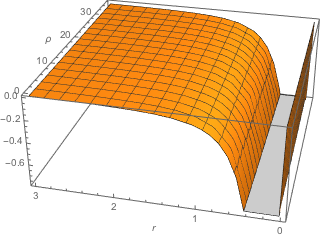
\includegraphics[width=0.45\textwidth]{figures/PartialDerivativeDiagram.png}
     \caption{Partial Derivative against $\rho$ and $r$: $ \frac{\partial \frac{\text{two-hop}(r)}{ \text{one-hop}(r)}}{\partial \rho, r} $ }
  \label{fig:partialderivativediagram}
\end{figure}
\end{quote}



\item
  - In eq. (27) and (28), it needs to be changed as 9/2 instead of 9.
  \highlighttext{Corrected--thank you!}  
  \item
- Figure 12 interferes to understanding the related contents. It is recommended to change
figure 12 referring the following figure,

\highlighttext{The reviewer has provided an excellent simplifying diagram. I have created a diagram similar
  (see \cref{fig:projectiondiagram})
  to theirs but retaining the numbering features, which are useful in the first place the
  figure is referenced, and in explaining the derivation of the inradius.
  I thank the reviewer for this improvement.}

\begin{figure}
     \centering
     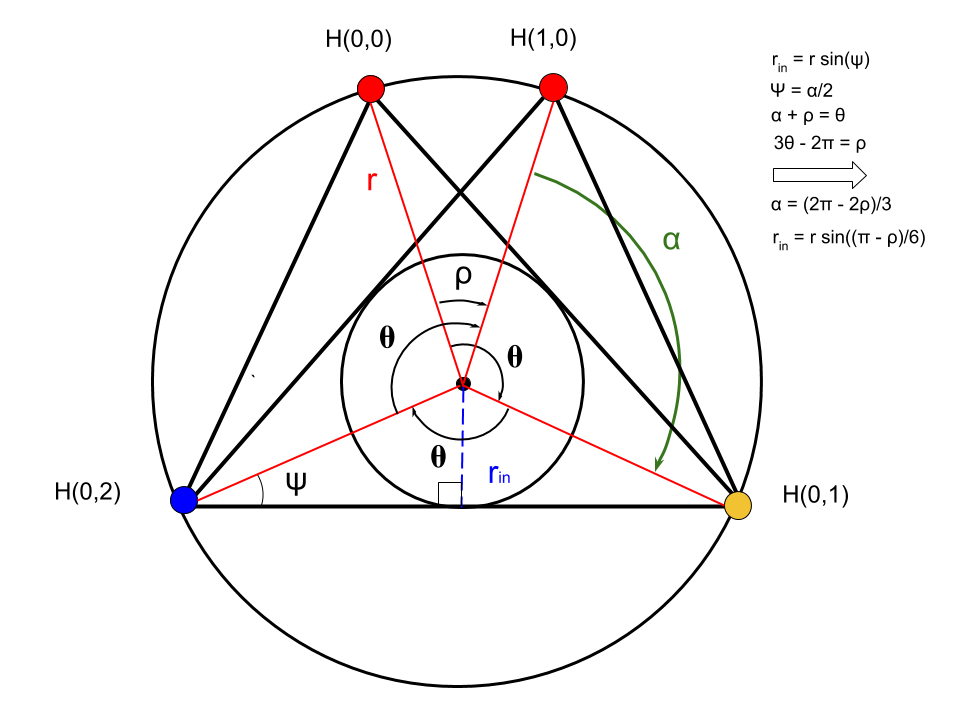
\includegraphics[width=0.45\textwidth]{figures/GeneralProjectionDiagramV2.png}
     \caption{General One-hop Projection Diagram}
  \label{fig:projectiondiagram}
\end{figure}

\item
- It would be great to add the snapshot and explanation showing the application of this
conclusion

\highlighttext{In order to more clearly tie this to the actual research robot for which it was developed,
  I have re-referenced the photograph which occurs early in the paper and modified the text:}

\begin{quote}
  \begin{figure}
  \centering
     \includegraphics[width=0.5\textwidth]{figures/MedCantedCropped.png}
     \caption{7-Tet Tetrobot in relaxed, or BC helix configuration}
     \includegraphics[width=0.5\textwidth]{figures/EquitetrabeamCropped.png}
     \caption{The Equitetrabeam: Fully Untwisted 7-Tet Tetrobot in Hexapod Configuration}
     \label{fig:tetrobot}
\end{figure}

A machine, such as \highlighttext{the} Tetrobot or a variable-geometry truss \highlighttext{ depicted in \cref{fig:tetrobot}}, that can change
the length of some of its members by $16\%$ can thus twist and untwist itself.
A completely regular Tetrobot can untwist itself to create a planar
face on the ground for locomotion \highlighttext{via standard gaits}.
\end{quote}

\end{itemize}


\section{Response to Reviewer \#2}

Title: A Continuum of Optimal Tetrahelices between the Boerdijk-Coxeter Helix and a Planar-faced Tetrahelix 

This paper proposed a method to transform the BC helix to Planar-faced tetrahelix by minimizing the difference between the longest and shortest edges, under some constraints. The author tried to explain his finding logically, and the background of the research is explained well. Also, the author shared the materials for this research at github. I have some comments for this paper as follows:

\begin{enumerate}

  \item
 I can see the organization of this paper is as follows: 
 Intro (2pages) – A designer’s formulation for the BC helix(2 pages) – Optimal tetrahelices are triple helix(3 pages) – Parameterizing tetrahelices via rail angle(2 pages) – The inradius(0.5 pages) – The Equitetrabeam (0.5 pages) – An Untwisted continuum (0.5 pages) – Conclusion
 \item 
   I think the author tried to explain all the findings but I think the organization of the paper should be revised to be emphasized carefully. Even for the researchers in this field, I am not convinced the paper is clearly written to emphasize the contribution well. Some sections can be combined, and the organization should be changed to emphasize the major contribution of this paper. I think this is the most significant point to improve the readability of the paper.

   \highlighttext{
     In order to address this, I have added the sentence below at the end of the introduction.
     }

   \highlighttext {
The remainder of this  paper:
\begin{enumerate}
\item provides a new formulation for the BC helix that is more natural for engineers,
\item defines a concept of minimum maximum edge-length optimality that maintains
  the structure as close to regularity as possible,
  \item proves that all
    optimal tetrahelices are in fact triple helices,
\item provides formulae for constructing optimal tetrahelices of different twists or for optimally
    transforming a
    robot from a twisted to a planar configuration in a way that maintains optimum regularity,
\item gives a formula for the inradius of an optimal tetrahelix,
\item describes a completely planar tetrahlix (the \emph{equitetrabeam}) useful as
  a structural beam or for applying standard robot gaits to a tetrahedral robot, and
\item discusses the continuum of optimal tetrahelices between the BC Helix and equitetrabeam.
  \end{enumerate}
}

  \item
    I think the explaining optimization part should be revised. For a certain optimization problem, I think mathematics definition or algorithmic explanation can be helpful to understand the problem quickly. I think the author should refer problem definition standards from other optimization papers to revise this.
    \highlighttext{
      In order to clarify the ``Optimal Tetrahelices are Triple Helices'' section as requested,
      I have provided a mathematical description of the optimization, and a more mathematical
      description of the definition of the tetrahelix.
      }


  \item    
    In my opinion, the problem definition and proof of theorems looks being done based on personal experiences. I recommend using mathematical derivation or expression if possible.
    \highlighttext{
      I believe the theorems are all true (and verified by computer experimentation) and that the proofs
      are rigorous. However, in deference to the reviewer I have significantly rewritten parts of them
      more formally in several places. Unfortunately, it is beyond my ability to make them completely formal
      in the space allowed in this paper. I hope readers will find them convincing at the available length.
      }

  \item    
    I think the demonstration by experiment can be helpful to understand the idea. Video attachment is recommended.
    \highlighttext{
I have included a public link to a video\cite{tetrahelixvideo} in the citations, and will upload the same video to the journal if appropriate.
\begin{quote}All math
developed here is available in JavaScript and demonstrated by an interactive
design website \url{https://pubinv.github.io/tetrahelix/}\cite{readtetrahelix}
\bf{and a video\cite{tetrahelixvideo}},
from which figs. 1 and 2 and later figures in this paper 
are taken.      
\end{quote}
    }

\end{enumerate}

Minors:

\begin{itemize}
  \item
    I am very confusing to the term ``An untwisted continuum'' and ``equitetrabeam.''
    \highlighttext{I have attempted to clarify this by adding the phrase:
      We call this the \emph{equitetrabeam}\textbf{, a portmanteau of ``equilateral tetrahedral beam''}.}
    Some other terminologies should be checked for 
    “Conincident” should be “coincident”
    \highlighttext{This has been corrected, thank you.}
\item
  Title is little bit not easy to be understood. “A continuum of optimal tetrahelices” can be changed to some other expression.
  \highlighttext{
    I have changed the title to:
 ``Transforming Optimal Tetrahelices between the Boerdijk-Coxeter Helix and a Planar-faced Tetrahelix''
}
\end{itemize}


\bibliographystyle{asmems4}
\bibliography{IEEEabrv,gluss}

\end{document}
